\documentclass{article}

\usepackage{multirow}
\usepackage{fancyhdr}
\usepackage{extramarks}
\usepackage{amsmath}
\usepackage{amsthm}
\usepackage{amsfonts}
\usepackage{tikz}
\usepackage[plain]{algorithm}
\usepackage{algpseudocode}
\usepackage{listings} 
\usepackage{neuralnetwork}
\usepackage{subfigure}
\usepackage[colorlinks,linkcolor=blue]{hyperref}
\usetikzlibrary{automata,positioning}

\usepackage{color}

\definecolor{dkgreen}{rgb}{0,0.6,0}
\definecolor{gray}{rgb}{0.5,0.5,0.5}
\definecolor{mauve}{rgb}{0.58,0,0.82}

\lstset{frame=tb,
  language=Python,
  aboveskip=3mm,
  belowskip=3mm,
  showstringspaces=false,
  columns=flexible,
  basicstyle={\small\ttfamily},
  numbers=none,
  numberstyle=\tiny\color{gray},
  keywordstyle=\color{blue},
  commentstyle=\color{dkgreen},
  stringstyle=\color{mauve},
  breaklines=true,
  breakatwhitespace=true,
  tabsize=3
}
%
% Basic Document Settings
%

\topmargin=-0.45in
\evensidemargin=0in
\oddsidemargin=0in
\textwidth=6.5in
\textheight=9.0in
\headsep=0.25in

\linespread{1.1}

\pagestyle{fancy}
\lhead{\hmwkAuthorName}
\chead{\hmwkClass\: \hmwkTitle}
\rhead{\firstxmark}
\lfoot{\lastxmark}
\cfoot{\thepage}

\renewcommand\headrulewidth{0.4pt}
\renewcommand\footrulewidth{0.4pt}

\setlength\parindent{0pt}

%
% Create Problem Sections
%

\newcommand{\enterProblemHeader}[1]{
    \nobreak\extramarks{}{Task \arabic{#1} continued on next page\ldots}\nobreak{}
    \nobreak\extramarks{Task \arabic{#1} (continued)}{Problem \arabic{#1} continued on next page\ldots}\nobreak{}
}

\newcommand{\exitProblemHeader}[1]{
    \nobreak\extramarks{Task \arabic{#1} (continued)}{Problem \arabic{#1} continued on next page\ldots}\nobreak{}
    \stepcounter{#1}
    \nobreak\extramarks{Task \arabic{#1}}{}\nobreak{}
}

\setcounter{secnumdepth}{0}
\newcounter{partCounter}
\newcounter{homeworkProblemCounter}
\setcounter{homeworkProblemCounter}{1}
\nobreak\extramarks{Task \arabic{homeworkProblemCounter}}{}\nobreak{}

%
% Homework Problem Environment
%
% This environment takes an optional argument. When given, it will adjust the
% problem counter. This is useful for when the problems given for your
% assignment aren't sequential. See the last 3 problems of this template for an
% example.
%
\newsavebox{\Taskname}
\newenvironment{homeworkProblem}[1][-1]{
    \ifnum#1>0
        \setcounter{homeworkProblemCounter}{#1}
    \fi
    \section{Task \arabic{homeworkProblemCounter}}
    \setcounter{partCounter}{1}
    \enterProblemHeader{homeworkProblemCounter}
}{
    \exitProblemHeader{homeworkProblemCounter}
}

%
% Homework Details
%   - Title
%   - Due date
%   - Class
%   - Section/Time
%   - Instructor
%   - Author
%

\newcommand{\hmwkTitle}{Assignment\ \#3}
\newcommand{\hmwkDueDate}{March 10, 2019}
\newcommand{\hmwkClass}{CSCI964 Computational Intelligence}
\newcommand{\hmwkClassTime}{2.14}
\newcommand{\hmwkClassInstructor}{Zhifeng Wang}
\newcommand{\hmwkAuthorName}{\textbf{Mei Wangzhihui}}
\newcommand{\hmwkAuthorNum}{\textbf{2019124044}}
%
% Title Page
%

\title{
    \vspace{2in}
    \textmd{\textbf{\hmwkClass:\ \hmwkTitle}}\\
    % \normalsize\vspace{0.1in}\small{Due\ on\ \hmwkDueDate\ at 3:10pm}\\
    % \vspace{0.1in}\large{\textit{\hmwkClassInstructor\ \hmwkClassTime}}
    \vspace{3in}
}

\author{\hmwkAuthorName\ \hmwkAuthorNum}
\date{}

\renewcommand{\part}[1]{\textbf{\large Part \Alph{partCounter}}\stepcounter{partCounter}\\}

%
% Various Helper Commands
%

% Useful for algorithms
\newcommand{\alg}[1]{\textsc{\bfseries \footnotesize #1}}

% For derivatives
\newcommand{\deriv}[1]{\frac{\mathrm{d}}{\mathrm{d}x} (#1)}

% For partial derivatives
\newcommand{\pderiv}[2]{\frac{\partial}{\partial #1} (#2)}

% Integral dx
\newcommand{\dx}{\mathrm{d}x}

% Alias for the Solution section header
\newcommand{\solution}{\textbf{\large Solution}}

% Probability commands: Expectation, Variance, Covariance, Bias
\newcommand{\E}{\mathrm{E}}
\newcommand{\Var}{\mathrm{Var}}
\newcommand{\Cov}{\mathrm{Cov}}
\newcommand{\Bias}{\mathrm{Bias}}

\begin{document}

\maketitle

\pagebreak

\begin{homeworkProblem}
  \subsection{Introduction to MNIST}
  The MNIST dataset is a handwritten digital picture dataset, a very popular experimental data set in machine learning, almost becoming a model. It is available at website \href{http://yann.lecun.com/exdb/mnist/}{THE MNIST DATABASE}, and it contains four parts:
  \begin{itemize}
    \item Training set images: train-images-idx3-ubyte.gz (9.9 MB, containing 60,000 samples)
    \item Training set labels: train-labels-idx1-ubyte.gz (29 KB, containing 60,000 labels)
    \item Test set images: t10k-images-idx3-ubyte.gz (1.6 MB, containing 10,000 samples)
    \item Test set labels: t10k-labels-idx1-ubyte.gz (5KB, containing 10,000 labels)
  \end{itemize}
  The MNIST dataset comes from the National Institute of Standards and Technology (NIST). Now do you know the origin of the name of this data set? M is the abbreviation of Modified. The training set is composed of numbers handwritten from 250 different people, of which 50\% are high school students and 50\% are from the staff of the Census Bureau. The test set is also the same proportion of handwritten digital data. Each picture is composed of 28x28 pixels, and each pixel is represented by a gray value. Here, the 28x28 pixels are expanded into a one-dimensional line vector (784 values ​​per line). The picture label is one-hot code: 0-9.

  MNIST's original black and white (dual horizontal) image size is standardized to fit a 20x20 frame while retaining its aspect ratio. As a result of the anti-aliasing technique used by the normalization algorithm, the resulting image contains gray levels. The center of mass pixel image is shifted, positioning the image in the center of the 28x28 field, thereby centering it in the 28x28 image, just like Figure \ref{fNNIST0}.

  \begin{figure}[h]
    \centering
    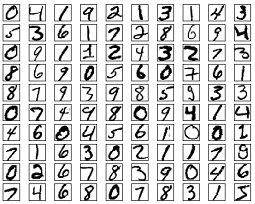
\includegraphics[width=0.5\textwidth]{image/blog_mnist}
    \caption{MNIST data sample}
    \label{fNNIST0}
  \end{figure}

  \subsection{Introduction of SOM}
  SOM stands for Self-Organizing Map and is an unsupervised learning neural network for feature detection. It simulates different characteristics of the division of nerve cells in different regions of the human brain, that is, different regions have different response characteristics, and this process is automatically completed. SOM is used to generate a low-dimensional space of training samples. It can convert complex non-linear statistical relationships between high-dimensional data into simple geometric relationships and display them in a low-dimensional manner. Therefore, it is usually used in dimensionality reduction problems. SOM is different from other artificial neural networks because they use competitive learning instead of error-related learning, while involving back propagation and gradient descent. In competitive learning, each will compete with each other to respond to a subset of input data(Figure \ref{SOMnet}).

  \begin{figure}[h]
    \centering
    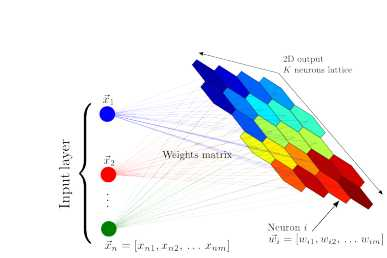
\includegraphics[width=0.5\textwidth]{image/SOM1}
    \caption{SOM architecture}
    \label{SOMnet}
  \end{figure}

  The training process is like the following Figure \ref{SOMtrain}. The purple area represents the distribution of training data, and the white grid represents the current training data extracted from the distribution. First, the SOM node is located anywhere in the data space. The node closest to the training data (highlighted in yellow) will be selected. It moves towards training data just like neighboring nodes in the grid. After many iterations, the grid tends to approximate this kind of data distribution.

  \begin{figure}[h]
    \centering
    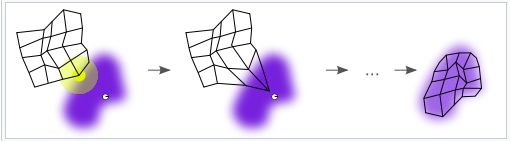
\includegraphics[width=0.5\textwidth]{image/SOM2}
    \caption{SOM training rocess}
    \label{SOMtrain}
  \end{figure}

  \subsection{Ordering and convergence}
  If the parameters are correctly initialized, we can start from the completely disordered initial state, and the SOM algorithm will gradually make the activation patterns obtained from the input space represent ordered. (However, it may end up in a metastable state where the feature map has topological defects.)

  There are two significant stages in this adaptive process:
  Ordering or self-organizing stage: During this period, the weight vectors are topologically sorted. Usually this will require up to 1000 iterations of the SOM algorithm, and careful selection of neighborhood and learning rate parameters needs to be considered.

  Convergence phase: During this period feature maps are fine tuned and provide accurate statistical quantization of the input space. Usually the number of iterations at this stage is at least 500 times the number of neurons in the network, and the parameters must be selected carefully.
  Here I set the number of ordering iterations as 1000, and the number of convergence iterations as 2000

  In my implementation, the ordering epoch is set to 1000 and convergence epoch is set to 2000, and the learning rate is set to 0.1.

  \subsection{Distance each epoch}
  The euclidean distance between its values in the t-th and (t+1)-th iterations convergence in a few epochs and then decrease slowly with fluctuation.
  \begin{figure}[h]
    \centering
    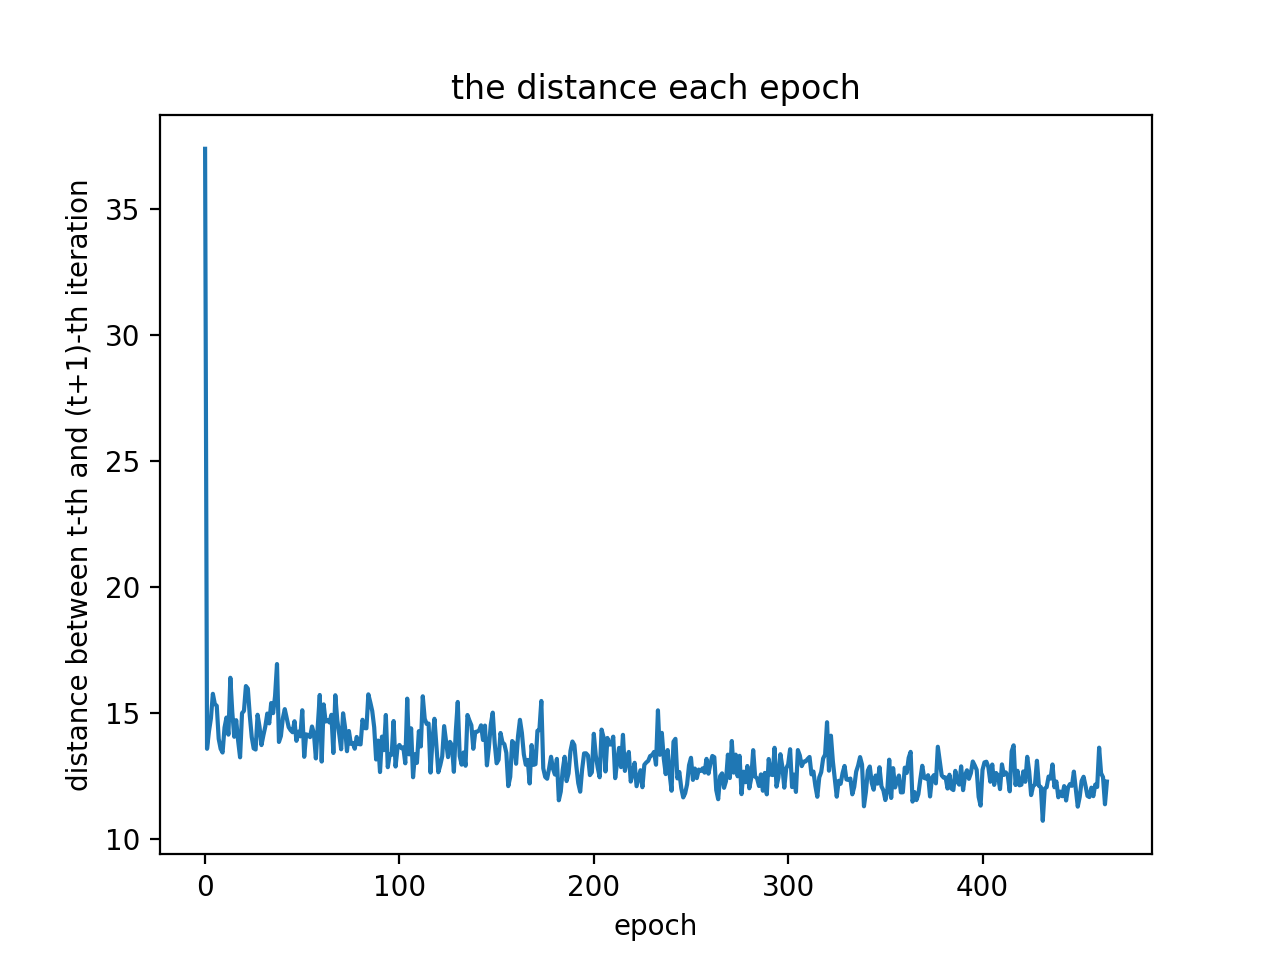
\includegraphics[width=0.5\textwidth]{image/dis}
    \caption{Distance each epoch}
    \label{dis}
  \end{figure}

  \subsection{2D lattices of three stages}
  \subsubsection{Initialization stage}
  \begin{figure}[H]
    \centering
    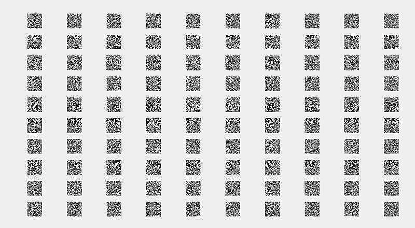
\includegraphics[width=1.0\textwidth]{image/somf1}
    \caption{Initialization stage}
    \label{somf1}
  \end{figure}

  \subsubsection{Between Initialization stage and Convergence stage}
  \begin{figure}[H]
    \centering
    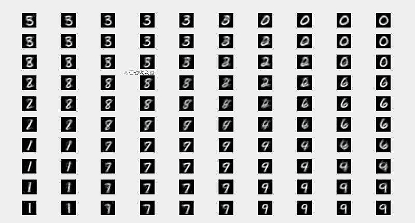
\includegraphics[width=1.0\textwidth]{image/somf2}
    \caption{Between Initialization stage and Convergence stage}
    \label{somf2}
  \end{figure}

  \subsubsection{Convergence stage}
  \begin{figure}[H]
    \centering
    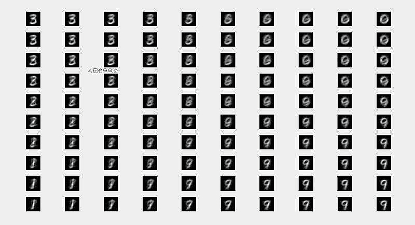
\includegraphics[width=1.0\textwidth]{image/somf3}
    \caption{Convergence stage}
    \label{somf3}
  \end{figure}

\end{homeworkProblem}

\begin{homeworkProblem}
  \subsection{Introduction to MNIST}
  The MNIST dataset is a handwritten digital picture dataset, a very popular experimental data set in machine learning, almost becoming a model. It is available at website \href{http://yann.lecun.com/exdb/mnist/}{THE MNIST DATABASE}, and it contains four parts:
  \begin{itemize}
    \item Training set images: train-images-idx3-ubyte.gz (9.9 MB, containing 60,000 samples)
    \item Training set labels: train-labels-idx1-ubyte.gz (29 KB, containing 60,000 labels)
    \item Test set images: t10k-images-idx3-ubyte.gz (1.6 MB, containing 10,000 samples)
    \item Test set labels: t10k-labels-idx1-ubyte.gz (5KB, containing 10,000 labels)
  \end{itemize}

  The MNIST dataset can be imported by TensorFlow API directly.
  \begin{lstlisting}
  import tensorflow as tf
  from tensorflow.keras import datasets, layers, models


  (train_images, train_labels), (test_images,test_labels) = datasets.mnist.load_data()
\end{lstlisting}
  \subsection{Multinomial logistic regression}
  \subsubsection{Defining network}
  The following code define a 3-layer network like Figure \ref{mlrnet}. The input dimention was flattened from $28\times 28$ to $784\times 1$ in Flatten layer. The Dense layer was full-connection layer. The Dropout layer was adopted to preventing overfitting by keeping neutrons hidden and unchanged in one training epoch with a certain probability. The tf.nn.softmax function converts these logits to "probabilities" for each class. The losses.SparseCategoricalCrossentropy loss takes a vector of logits and a True index and returns a scalar loss for each example. Finally, set the model's optimizer to Adam (an optimizer that can adjust the learning rate adaptively), set loss function to SparseCategoricalCrossentropy and metrics to accuracy.
  \begin{lstlisting}
  model = tf.keras.models.Sequential([
    tf.keras.layers.Flatten(input_shape=(28, 28)),
    tf.keras.layers.Dense(128, activation='relu'),
    tf.keras.layers.Dropout(0.2),
    tf.keras.layers.Dense(10)
])
loss_fn = tf.keras.losses.SparseCategoricalCrossentropy(from_logits=True)
model.compile(optimizer='adam', loss=loss_fn, metrics=['accuracy'])
\end{lstlisting}
  \begin{figure}[h]
    \centering
    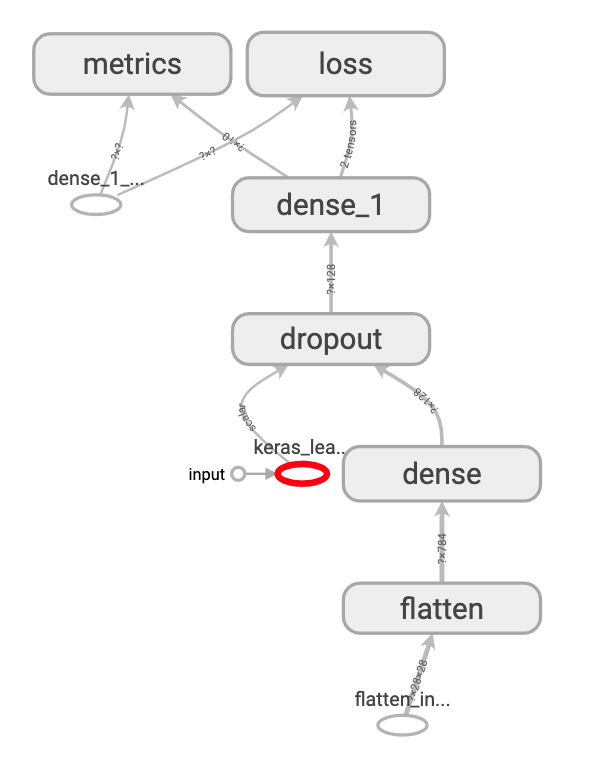
\includegraphics[width=0.2\textheight]{image/mlrnet}
    \caption{Multinomial logisticre gression network architecture}
    \label{mlrnet}
  \end{figure}

  \subsubsection{Training network}
  The following code training the neural network. We also applied tensorboard to visualize the trainging process, like Figure \ref{epoch_accuracy}.
  \begin{lstlisting}
model.fit(x_train,
        y_train,
        epochs=5,
        validation_data=(x_test, y_test),
        callbacks=[tensorboard_callback])
\end{lstlisting}
  \begin{figure}[h]
    \centering
    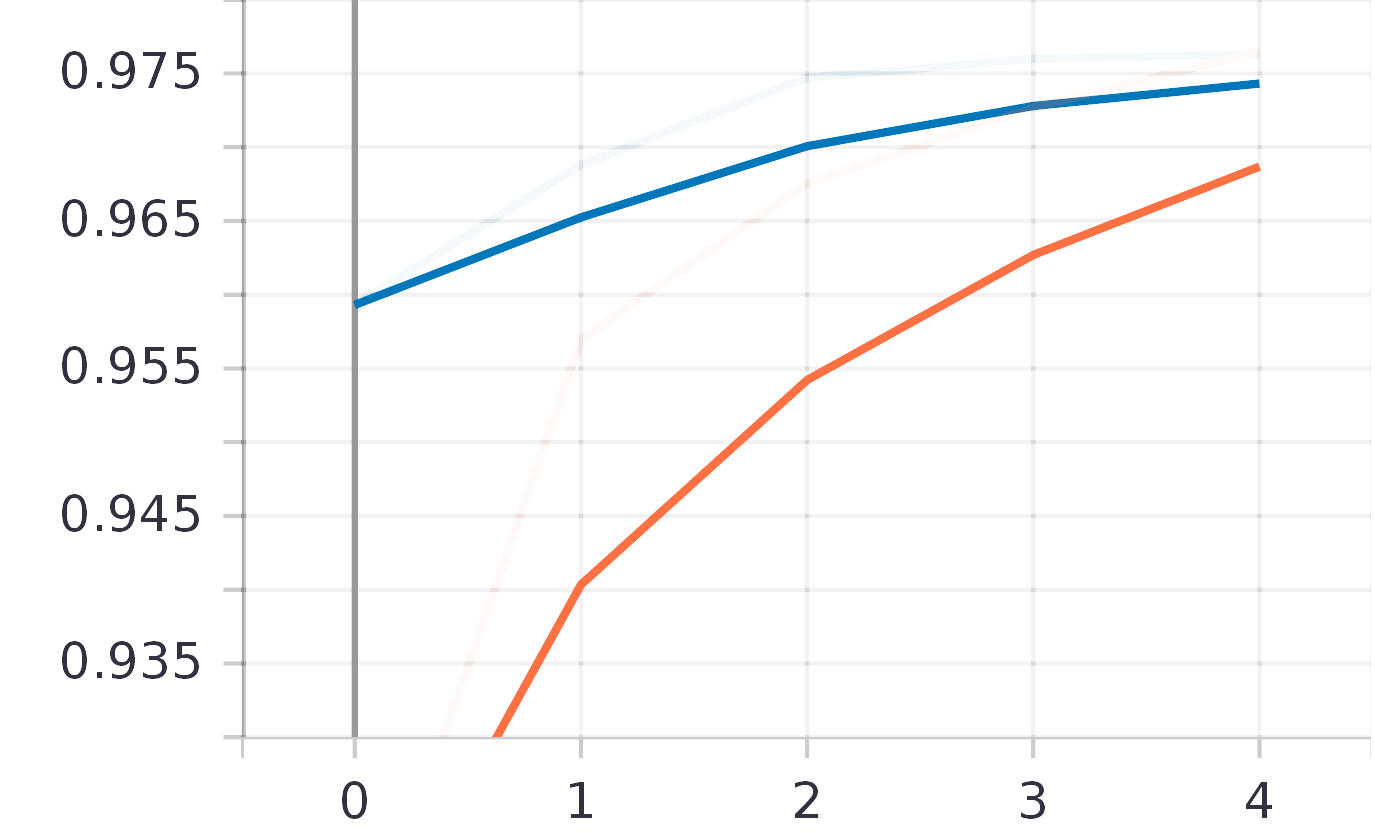
\includegraphics[width=0.4\textwidth]{image/epoch_accuracy}
    \caption{Epoch accuracy of training set and test set}
    \label{epoch_accuracy}
  \end{figure}
  \subsubsection{Test}
  The following code test the neural network's accuracy.
  \begin{lstlisting}
model.evaluate(x_test, y_test, verbose=2)
\end{lstlisting}
  \subsubsection{Tuning}
  As we change batch size, the graph down pan down like Figure \ref{epoch_accuracy_bs}.
  \begin{figure}[h]
    \centering
    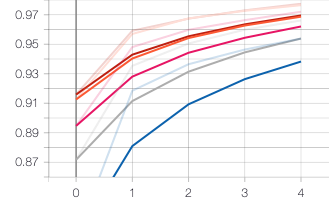
\includegraphics[width=0.4\textwidth]{image/epoch_accuracy_bs}
    \caption{Epoch accuracy of different batch size}
    \label{epoch_accuracy_bs}
  \end{figure}

  As we change optimizer and learning rate, the graphs vary like Figure \ref{epoch_accuracy_op}.
  \begin{figure}[h]
    \centering
    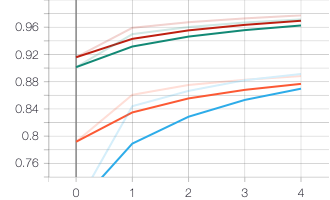
\includegraphics[width=0.4\textwidth]{image/epoch_accuracy_op}
    \caption{Epoch accuracy of different optimizer}
    \label{epoch_accuracy_op}
  \end{figure}


  \subsection{Multi-layer neural network}
  \subsubsection{Defining network}
  The following code define a basic neural network model. The first layer is a convolutional layer with 32 3x3 convolution kernel and RELU activation function. The second layer is a Flatten layer to flatten multi-dimensional input to a 1d-vector. The third is a hidden full-connection layer with RELU as activation function. The final layer is a output layer to output a one-hot encoding vector.
  \begin{lstlisting}

class MyModel(Model):
    def __init__(self):
        super(MyModel, self).__init__()
        self.conv1 = Conv2D(32, 3, activation='relu')
        self.flatten = Flatten()
        self.d1 = Dense(128, activation='relu')
        self.d2 = Dense(10)

    def call(self, x):
        x = self.conv1(x)
        x = self.flatten(x)
        x = self.d1(x)
        return self.d2(x)


model = MyModel()

loss_object = tf.keras.losses.SparseCategoricalCrossentropy(from_logits=True)

optimizer = tf.keras.optimizers.Adam()

train_loss = tf.keras.metrics.Mean(name='train_loss')
train_accuracy = tf.keras.metrics.SparseCategoricalAccuracy(
    name='train_accuracy')

test_loss = tf.keras.metrics.Mean(name='test_loss')
test_accuracy = tf.keras.metrics.SparseCategoricalAccuracy(
    name='test_accuracy')
  
\end{lstlisting}

  \subsubsection{Training and testing}
  The following code applied the training process and testing process.
  \begin{lstlisting}
@tf.function
def train_step(images, labels):
    with tf.GradientTape() as tape:
        # training=True is only needed if there are layers with different
        # behavior during training versus inference (e.g. Dropout).
        predictions = model(images, training=True)
        loss = loss_object(labels, predictions)
    gradients = tape.gradient(loss, model.trainable_variables)
    optimizer.apply_gradients(zip(gradients, model.trainable_variables))

    train_loss(loss)
    train_accuracy(labels, predictions)


@tf.function
def test_step(images, labels):
    # training=False is only needed if there are layers with different
    # behavior during training versus inference (e.g. Dropout).
    predictions = model(images, training=False)
    t_loss = loss_object(labels, predictions)

    test_loss(t_loss)
    test_accuracy(labels, predictions)

    EPOCHS = 5

for epoch in range(EPOCHS):
    # Reset the metrics at the start of the next epoch
    train_loss.reset_states()
    train_accuracy.reset_states()
    test_loss.reset_states()
    test_accuracy.reset_states()

    for images, labels in train_ds:
        train_step(images, labels)

    for test_images, test_labels in test_ds:
        test_step(test_images, test_labels)

    template = 'Epoch {}, Loss: {}, Accuracy: {}, Test Loss: {}, Test Accuracy: {}'
    print(
        template.format(epoch + 1, train_loss.result(),
                        train_accuracy.result() * 100, test_loss.result(),
                        test_accuracy.result() * 100))
\end{lstlisting}

\subsubsection{Tuning}
Tune the size of hidden layer, the accuracy and loss change like this Figure \ref{nnal}.

\begin{figure}[h]
  \centering
  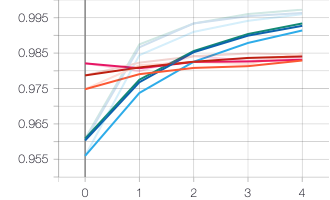
\includegraphics[width=0.4\textwidth]{image/nnaccuracy_hl}
  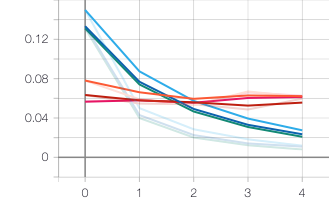
\includegraphics[width=0.4\textwidth]{image/nnloss_hl}
  \caption{Epoch accuracy/loss of different hidden layer size}
  \label{nnal}
\end{figure}

Tune the size of convolution kernel, the test accuracy increase and test loss decrease. See Figure \ref{nnks}.

\begin{figure}[h]
  \centering
  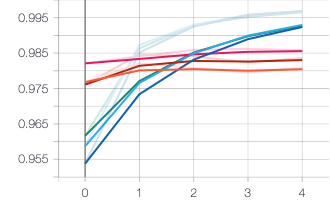
\includegraphics[width=0.4\textwidth]{image/nn_acc_ks}
  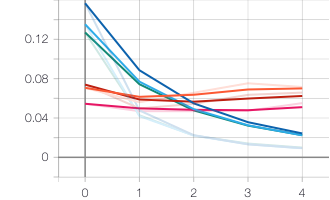
\includegraphics[width=0.4\textwidth]{image/nnloss_ks}
  \caption{Epoch accuracy/loss of different convolution kernel size}
  \label{nnks}
\end{figure}

\subsection{Cell image classification}
\subsubsection{a}
The classification technique is deep Convolutional Neural Network(CNN). 

The toolboxes is TensorFlow and TensorBoard.

The language is Python.
\subsubsection{b}
I applied CNN to this task. The network is a 22-layer-network with 15 convolutional layers, 4 pooling layer(MaxPooling) and 3 fully connected layers. Like Figure \ref{dcnnt}. The parameters of $k$, $s$ and $p$ denote the kernel size, stride, and padding size, respectively.
\begin{figure}[h]
  \centering
  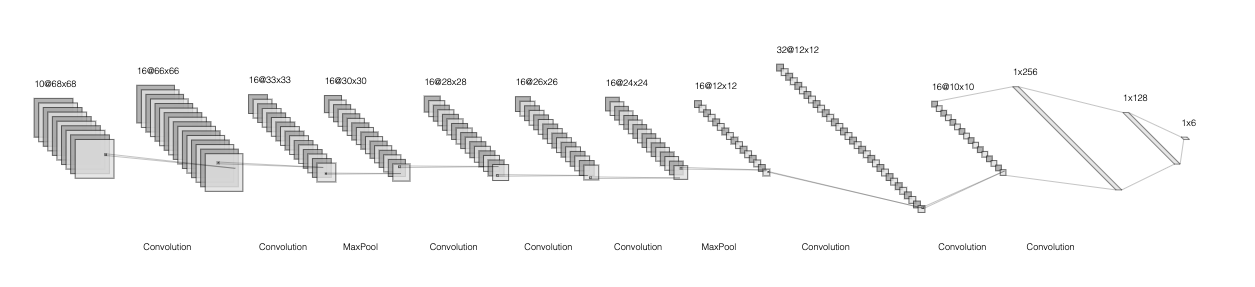
\includegraphics[width=1.0\textwidth]{image/dcnnt}
  \caption{The architecture of the network}
  \label{dcnnt}
\end{figure}

\subsubsection{c}
I applied gray level stretch to normalize the image intensities like Eq.\ref{eq1} 
\begin{equation}
  g=\frac{(f-\min (f)) \times 255}{\max (f)-\min (f)} \label{eq1}
\end{equation}
where $f$ is the input image pixel gray level and $g$ is the output pixel gray level.

Then, I applied data augmentation to the dataset. Data augmentation is a useful method for training CNN on small datasets. The images of different cell patterns in training set were rotated with different angles like Table \ref{datd}.

% Please add the following required packages to your document preamble:
% \usepackage{multirow}
% Please add the following required packages to your document preamble:
% \usepackage{multirow}
\begin{table}[H]
  \resizebox{\textwidth}{!}{
  \begin{tabular}{l|l|l|l|l|l|l|l|l}
  Patterns    & No. of Images & Training set for CNN & Rotation degree 1   & No. After Rotation & Rotation degree 2   & No. After Rotation & Rotation degree 3   & No. After Rotation \\ \hline
  Golgi       & 721           & 463                  & 24                  & 6945               & 12                  & 13890              & 6                   & 27780              \\ \hline
  Homogeneous & 2494          & 1596                 & \multirow{5}{*}{72} & 7980               & \multirow{5}{*}{36} & 15960              & \multirow{5}{*}{18} & 31920              \\ \cline{1-3} \cline{5-5} \cline{7-7} \cline{9-9} 
  Speckled    & 2831          & 1812                 &                     & 9060               &                     & 18120              &                     & 36240              \\ \cline{1-3} \cline{5-5} \cline{7-7} \cline{9-9} 
  Nucleolar   & 2598          & 1663                 &                     & 8315               &                     & 16630              &                     & 33260              \\ \cline{1-3} \cline{5-5} \cline{7-7} \cline{9-9} 
  Centromere  & 2741          & 1754                 &                     & 8770               &                     & 17540              &                     & 35080              \\ \cline{1-3} \cline{5-5} \cline{7-7} \cline{9-9} 
  NuMem       & 2208          & 1413                 &                     & 7065               &                     & 14130              &                     & 28260              \\ \hline
  Total       & 13596         & 8701                 &                     & 48135              &                     & 96270              &                     & 192540            
  \end{tabular}}
  \caption{Data augmentation to dataset}
  \label{datd}
\end{table}

% \begin{figure}[H]
%   \centering
%   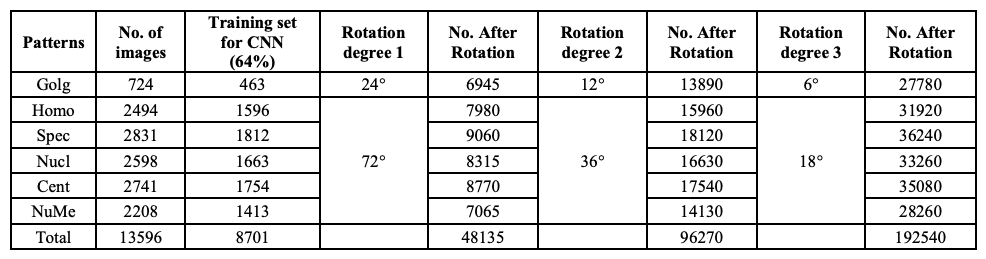
\includegraphics[width=1.0\textwidth]{image/dataau}
%   \caption{Data augmentation to dataset}
%   \label{dataau}
% \end{figure}

\subsubsection{d}
We choose convolutional kernel like $1\times 1$ and $3\times 3$ as they require less parameters and computational loss. Besides, $1\times 1$ kernel can reduce or add the dimension of feature map and integrate channel information of feature map. Each convolution layer is followed by a nonlinear activation layer with the activation function PreLU as Eq.\ref{prelu}, where $\theta$ is a parameter in learning process. On the side, $2\times 2$ max pooling is employed to decrease the dimension of feature maps. At the end of the proposed network, two fully-connected layers and one softmax layer are employed to classify cell images into six categories. To prevent the network from overfitting, I applied 0.5 dropout layer to it.  
\begin{equation}
  F=max(\theta x, x) \label{prelu}
\end{equation}

\subsubsection{e}
% The training accuracy of rotation degree 1 is 98.69\%, rotation degree 2 is 99.36\% and rotation degree 3 is 99.57\%. 

% The validation accuracy of rotation degree 1 is 96.33\%, rotation degree 2 is 98.73\% and rotation degree 3 is 99.34\%. 

The accuracy performance is like Table \ref{tb1}.
\begin{table}[H]
  \centering
  \begin{tabular}{|l|l|l|l|}
  \hline
       & Rotation degree 1 & Rotation degree 2 & Rotation degree 3 \\ \hline
      Training & 98.69 & 99.36 & 96.33 \\ \hline
      Validation & 96.33 & 98.73 & 99.34 \\ \hline
  \end{tabular}
  \caption{The training accuracy}
  \label{tb1}
\end{table}

% We applied two evaluation metrics for classification accuracy as $ACA$ and $MCA$.

% \begin{equation}
%   ACA=\frac{R}{N}
% \end{equation}
% where $R$ stands for the total right classification numbers of total cell images $N$.

% \begin{equation}
%   MCA=\frac{1}{n} \sum_{k=1}^{n} C C R_{k}
% \end{equation}
% where $CCR_k$ is the classification accuracy of class $k$ and $n$ stands for the number of cell classes.
\subsubsection{f}


The final accuracy performance is like Table \ref{TBL2}.

\begin{table}[H]
  \centering
  \begin{tabular}{|l|l|l|l|}
  \hline
  Rotation degree 1 & Rotation degree 2 & Rotation degree 3 \\ \hline
  95.33 & 98.02 & 98.17 \\ \hline
  \end{tabular}
  \caption{The final accuracy performance}
  \label{TBL2}
\end{table}

\subsubsection{g}
We can generate the output of each layer and get the following results Figure \ref{cnn1} and \ref{cnn2}.
\begin{figure}[h]
  \centering
  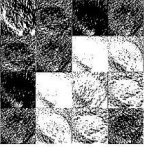
\includegraphics[width=0.2\textwidth]{image/cnn1}
  \caption{Feature maps from first convolution layer}
  \label{cnn1}
\end{figure}
\begin{figure}[h]
  \centering
  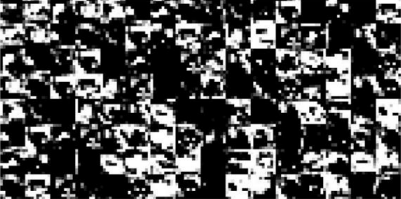
\includegraphics[width=0.4\textwidth]{image/cnn2}
  \caption{Feature maps from last convolution layer}
  \label{cnn2}
\end{figure}

It seems to be that the first convolution layer reveal the edge of initial image, and features learned by the last layer is abstract and clear.

We can also draw the conclusion that more data generate better accuracy from the final accuracy, as the number of data increase with degree.


\end{homeworkProblem}
\end{document}

